\documentclass[14pt,a4paper]{article}
\usepackage[14pt]{extsizes}
\usepackage[left=1.5cm, right=1.5cm, top=1.5cm, bottom=1.5cm]{geometry}
\usepackage[utf8]{inputenc}
\usepackage[T2A]{fontenc}
\usepackage[english, russian]{babel}
\usepackage{amsmath,amsfonts,amssymb,amsthm,mathtools}
\usepackage{amsfonts}
\usepackage{amssymb}
\usepackage{titleps}
\usepackage{hyperref}
\usepackage{float}
\usepackage{graphicx}
\usepackage{multirow}
\usepackage{hhline}
\usepackage{wrapfig}
\usepackage{tikz}
\usepackage{pgfplots}
\usepackage{xcolor}
\usepackage{subfig}
\usepackage{upgreek}
\usepackage{bm}
\usepackage{longtable}



\begin{document}

\begin{titlepage}
	\begin{center}
		\large 	Московский физико-технический институт \\
		\vspace{0.2cm}

		\vspace{4.5cm}
		Лабораторная работа № 4.3.2 \\ \vspace{0.2cm}
		\large (Общая физика: оптика) \\ \vspace{0.2cm}
		\LARGE \textbf{Дифракция света на ультразвуковой волне}
	\end{center}
	\vspace{2.3cm} \large

	\begin{center}
		Работу выполнил: \\
        Лазарь Владислав, группа Б01-202




	\end{center}

	\begin{center} \vspace{110mm}
		г. Долгопрудный \\
		 2024 год
	\end{center}
\end{titlepage}


\newpage

\paragraph*{Цель работы:} изучение дифракции света на синусоидальной акустической решетке и наблюдение фазовой решетки методом темного поля.

	\paragraph*{Оборудование:} оптическая скамья, осветитель, два длиннофокусных объектива, кювета с жидкостью, кварцевый излучатель с микрометрическим винтом, генератор звуковой частоты, линза, вертикальная нить на рейтере, микроскоп.

	\section*{Теоретическое введение}

	В работе используются оптическая скамья, осветитель, два длиннофокусных объектива, кювета с жидкостью, кварцевый излучатель с микрометрическим винтом, генератор звуковой частоты, линза, горизонтальная нить на рейтере, микроскоп.

	При прохождении ультразвуковой волны через жидкость в ней возникают периодические неоднородности коэффициента преломления, создается фазовая решетка, которую мы считаем неподвижной ввиду малости скорости звука относительно скорости света. Показатель
	преломления n изменяется по закону:

	\begin{equation}\label{}
	n = n_0 (1 + m \cos \Omega x)
	\end{equation}

	Здесь $ \Omega = 2 \pi / \Lambda $ --- волновое число для ультразвуковой волны, $ m $ --- глубина модуляции $ n $ $ (m \ll 1 $).

	Положим фазу $ \phi $ колебаний световой волны на передней стенке кюветы равной нулю, тогда на задней поверхности она равна:

	\begin{equation}\label{}
	\phi  = k n L = \phi_0 (1 + m \cos \Omega x)
	\end{equation}

	Здесь $ L $ --- толщина жидкости в кювете, $ k = 2 \pi / \lambda $ --- волновое число для света.

	После прохождения через кювету световое поле есть совокупность плоских волн, распространяющихся под углами $ \theta $, соответствующими максимумам в дифракции Фраунгофера:

\begin{equation}\label{}
	\Lambda \sin \theta_m = m \lambda
\end{equation}

	Этот эффект проиллюстрирован на рисунке 1.
	\begin{figure}[h!]
		\centering
		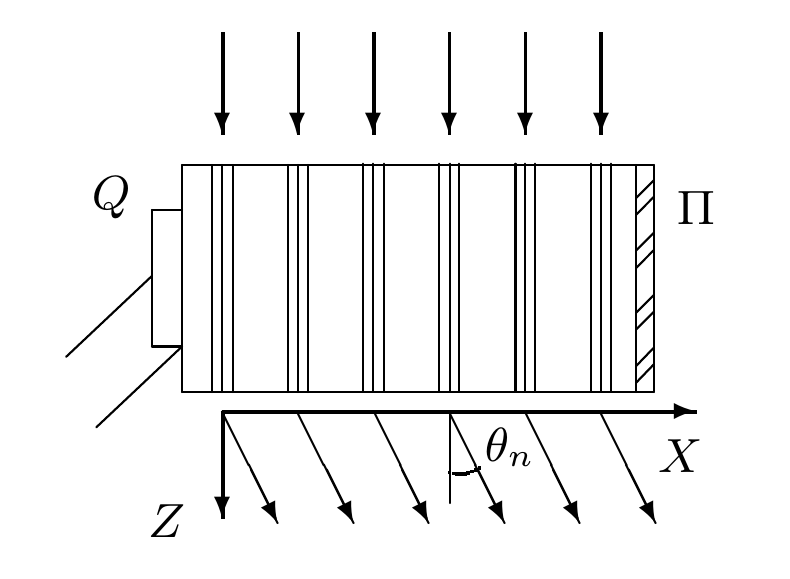
\includegraphics[width=0.3\textwidth]{Images/difraction.png}
		\caption{Дифракция световых волн на акустической решетке}
		\label{diff}
	\end{figure}

\newpage

	Зная положение дифракционных максимумов, по формуле (1) легко определить длину ультразвуковой волны, учитывая малость $ \theta $: $ \sin \theta \approx \theta \approx l_m /F  $, где $ l_m $ --- расстояние от нулевого до последнего видимого максимума, $ F $ --- фокусное расстояние линзы. Тогда получим:

	\begin{equation}\label{}
	 \Lambda = m \lambda F/ l_m
	\end{equation}
	Скорость ультразвуковых волн в жидкости, где $ \nu $ --- частота колебаний излучателя:

\begin{equation}\label{}
	v = \Lambda \nu
\end{equation}

    \section*{Метод фазового контраста и тёмного поля. } Рассмотрим проблему визуализации фазовых объектов, которую можно решить, используя метод фазового контраста, предложенный Цернике. Пусть фазовый объект — тонкая прозрачная пластинка, имеющая разный в разных точках показатель преломления (или толщину), но не изменяющая амплитуду прошедшей волны, находится во входной плоскости П1 оптической системы.

    \begin{figure}[H]
		\centering
		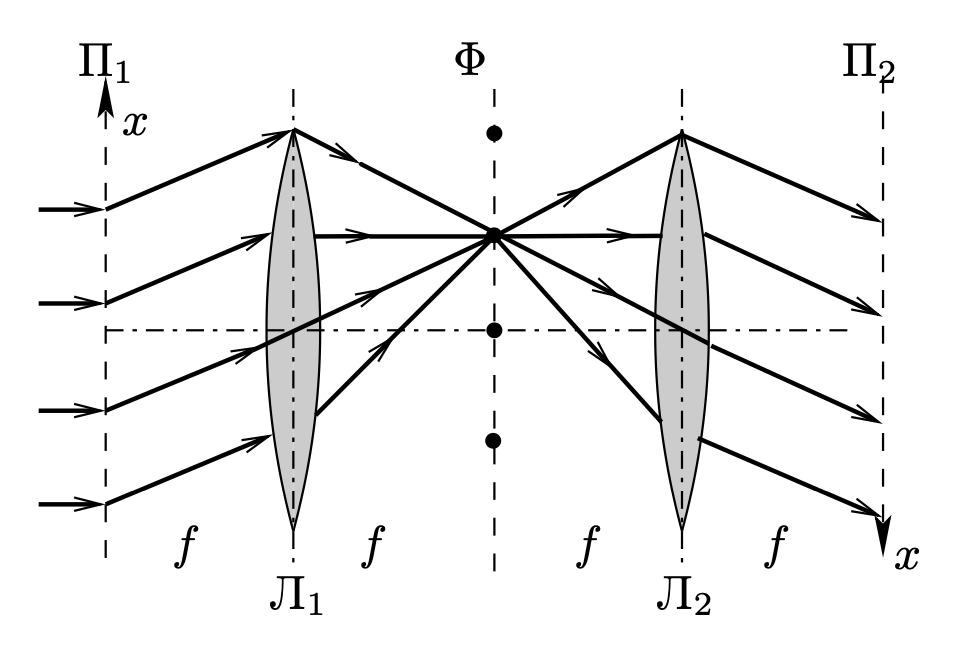
\includegraphics[width=0.6\textwidth]{Images/4f.png}
		\label{diff}
	\end{figure}

    Если оптическая система идеальна, в плоскости П2 мы наблюдаем равномерную засветку: информация о фазовой структуре предмета потеряна, фазовый объект невидим.

    Для визуализации фазового объекта Цернике предложил установить в фурье-плоскости, на оптической оси, маленькую фильтрующую пластинку, которая, не изменяя амплитуды прошедшей волны, вносит фазовую задержку, равную $\pi/2$.

    В методе тёмного поля вместо фазовой пластинки в фурье-плоскости на оптической оси устанавливается непрозрачный маленький экран.


\section*{Определение скорости ультразвука по дифракционной картине}

Схема установки приведена на рисунке 2. Источник света Л через светофильтр Ф и конденсор К освещает вертикальную щель $ S $, находящуюся в фокусе объектива $ O_1 $. После объектива параллельный световой пучок проходит через кювету С перпендикулярно акустической решетке, и дифракционная картина собирается в фокальной плоскости объектива $ O_2 $ , наблюдается при помощи микроскопа М.

Предварительную настройку установки произведем в соответствии с инструкцией с зеленым фильтром, далее в работе используется красный.

	\begin{figure}[H]
	\centering
	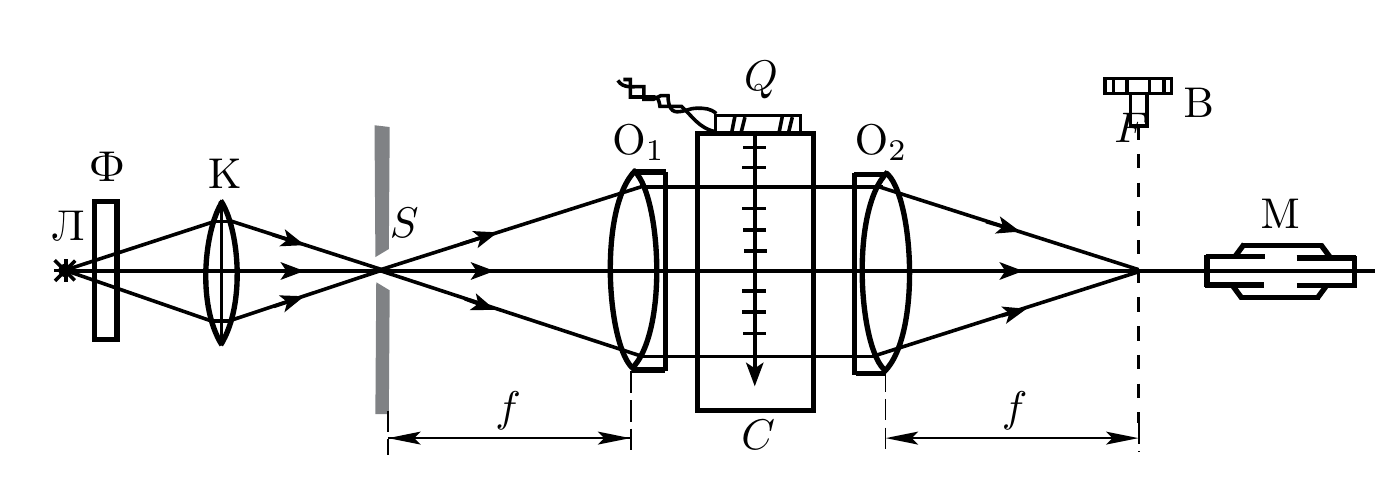
\includegraphics[width=0.7\textwidth]{Images/shema1.png}
	\caption{Схема для наблюдения дифракции на акустической решетке}
	\label{shema1}
\end{figure}

\section*{Определение скорости ультразвука методом темного поля}

Для наблюдения акустической решетки используется метод темного поля, который заключается в устранении центрального дифракционного максимума с помощью непрозрачного экрана. Схема установки показана на рисунке 7.

	\begin{figure}[H]
	\centering
	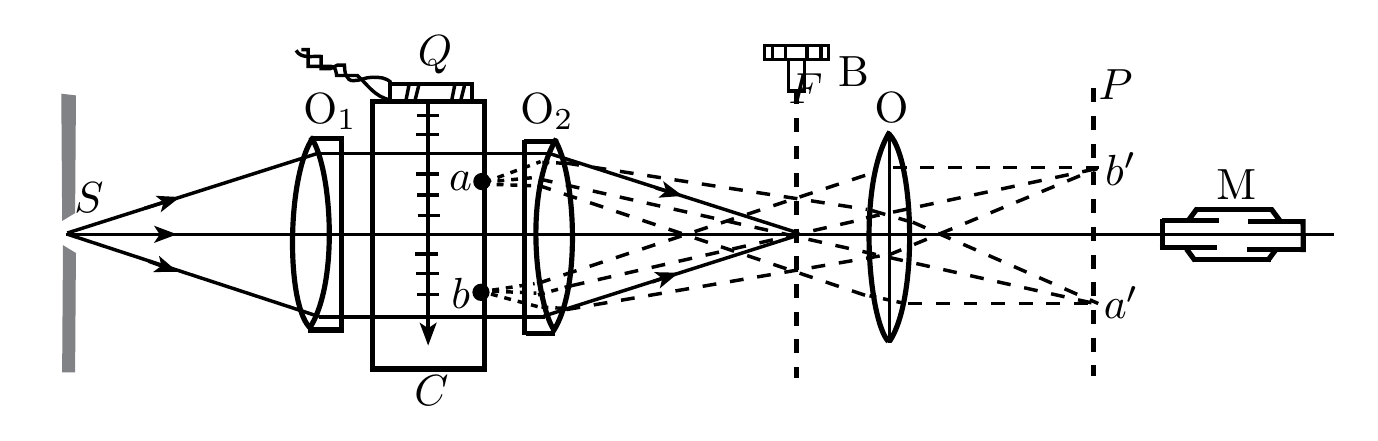
\includegraphics[width=0.7\textwidth]{Images/shema2.png}
	\caption{Схема для наблюдения дифракции методом темного поля}
	\label{shema2}
\end{figure}

Приставим к задней стенке (для светового луча) кюветы стеклянную пластинку с миллиметровыми делениями; сфокусируем микроскоп на изображение пластинки. Определим цену деления окулярной шкалы микроскопа, совместив ее с миллиметровыми делениями: в 6 делениях миллиметровой шкалы убирается 100 маленьких делений окулярной. Значит, цена деления окулярной шкалы: $ C = $ 0,06 мм.


\section*{Ход работы}
Данные с установки: \\
$\lambda_\text{кр} = 6400 \pm 200 \ \text{Å},$ \quad $f_1 = 94 \ \text{см},$ \quad $f_2 = 28 \ \text{см},$ \quad $f = 110 \ \text{см}.$
\subsection*{Определение скорости ультразвука по дифракционной картине}
\begin{itemize}
    \item цена деления лимба равна 10 мкм
    \item один оборот лимба равен 50 делениям
    \item максимальное перемещение излучателя --- 2 мм
\end{itemize}
\paragraph*{Оценка по порядку величины скорости ультразвука в дифракционной решётке \\}
После построения и настройки установки, изображённой на рис. 3, найдём рабочую частоту --- частоту, при которой видно наибольшее количество дифракционных полос: $\nu = 1.046$ \ МГц (при этой частоте видно 7 полос). А также оценим по порядку величины скорость звука как удвоенное расстояние между наиболее чёткими дифракционными картинами:
n = 160 делений.
Тогда длина волны будет равна:
\[
\Lambda = 10n = 1600 \ \text{мкм} = 1.6 \ \text{мм} ,
\]
Соответственно для погрешности $\Lambda$:
\[
\sigma_{\Lambda} = \Lambda \frac{\sigma_{n}}{n} = 0.01 \ \text{мм},
\]
Теперь можем оценить скорость ультразвуковой волны, зная длину волны:
\[
v = \Lambda\nu = 1673.6 \ \text{м/с},
\]
И выражение для погрешности $\sigma_v$:
\[
\sigma_v = v \sqrt{\left ( \frac{\sigma_{\Lambda}}{\Lambda} \right ) ^2 + \left ( \frac{\sigma_{\nu}}{\nu} \right ) ^2} = 10.6 \ \text{м/с},
\]
Итого:
\[
\boxed{v = (1673.6 \pm 10.6) \ \text{м/с}.}
\]

\newpage

\paragraph*{Точный метод нахождения скорости ультразвука в дифракционной решётке \\}
Измерим положение дифракционных полос $x_m$ в зависимости от номера полосы. Повторим измерения для нескольких частот, на которых четко видна дифракционная картина. Результаты занесем в таблицу:

\begin{table}[H]
    \centering
    \begin{tabular}{|l|l|l|l|l|l|}
    \hline
    \multicolumn{2}{|c|}{$\nu=1.08 \ \text{МГц}$} & \multicolumn{2}{c|}{$\nu=1.94 \ \text{МГц}$} & \multicolumn{2}{c|}{$\nu=3.2 \ \text{МГц}$} \\ \hline
        $m$ & $x_m, \ \text{мкм}$ & $m$ & $x_m, \ \text{мкм}$ & $m$ & $x_m, \ \text{мкм}$ \\ \hline
        -3 & -140 & -2  & 150  & -1  & 260  \\ \hline
        -2 & -30  & -1  & 405  & 0   & 630  \\ \hline
        -1 & 90   & 0   & 635  & 1   & 1000 \\ \hline
        0  & 228  & 1   & 850  & --- & ---  \\ \hline
        1  & 370  & 2   & 1090 & --- & ---  \\ \hline
        2  & 490  & --- & ---  & --- & ---  \\ \hline
        3  & 605  & --- & ---  & --- & ---  \\ \hline
    \end{tabular}
\caption{Результаты измрений координат дифракционных полос}
\end{table}

По результам измерений построим графики. Здесь $\Delta x_m = l_m$ --- расстояние от нулевого максимума до $m$-того максимума.

Находим $v$:
\[
v = \nu mf \frac{\lambda}{l_m} = \nu f \frac{\lambda}{k}
\]
В таблицу 2 занесём полученные коэффициенты наклона из графиков и скорость, посчитанную по формуле выше, учитывая, что погрешности равны:
\[
\sigma_v = v \sqrt{\left ( \frac{\sigma_{\lambda}}{\lambda} \right ) ^2 + \left ( \frac{\sigma_{\nu}}{\nu} \right ) ^2 + \left ( \frac{\sigma_{k}}{k} \right ) ^2}
\]

\begin{figure}[H]
    	\centering
    	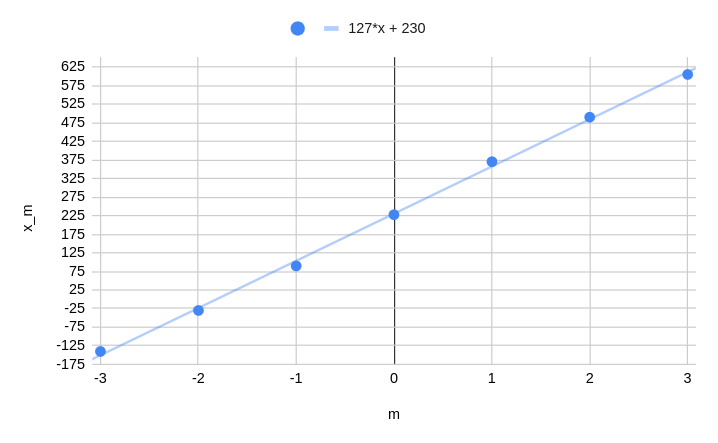
\includegraphics[width=0.9\textwidth]{Images/plot_1.png}
    	\label{shema1}
    \end{figure}
\begin{figure}[H]
    	\centering
    	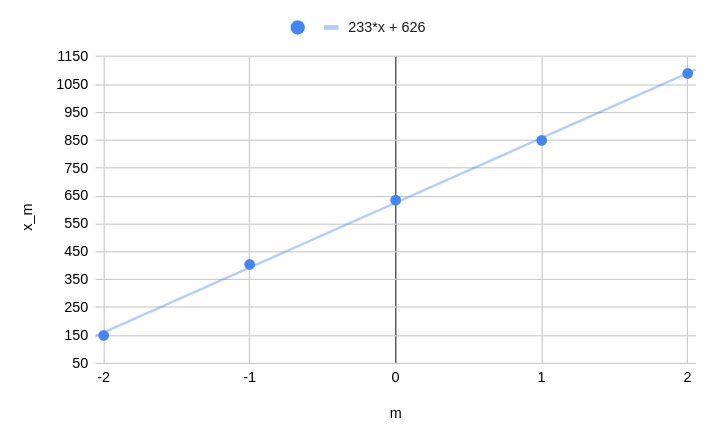
\includegraphics[width=0.9\textwidth]{Images/plot_2.png}
    	\label{shema1}
    \end{figure}
\begin{figure}[H]
    	\centering
    	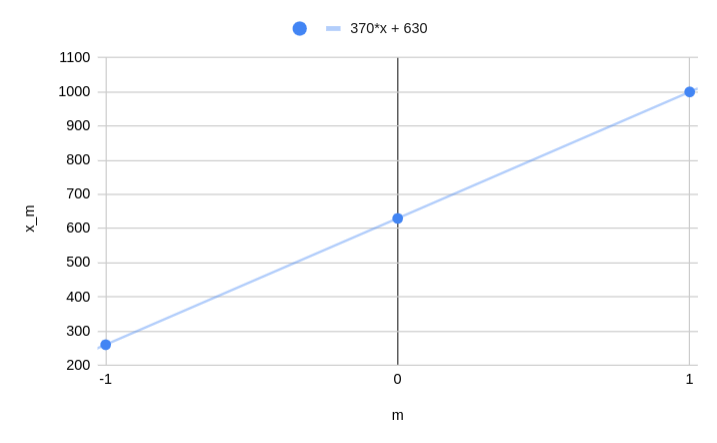
\includegraphics[width=0.9\textwidth]{Images/plot_3.png}
    	\label{shema1}
\end{figure}

\begin{table}[!ht]
    \centering
    \begin{tabular}{|l|l|l|l|}
    \hline
        $\nu, \ \text{МГц}$ & 1.08 & 1.94 & 3.2 \\ \hline
        $k$ & 127 $\pm$ 2& 233 $\pm$ 4& 370 $\pm$ 0  \\ \hline
        $v, \ \text{м/c}$& 1524 $\pm$ 55 & 1492 $\pm$ 58 & 1550  $\pm$ 62\\ \hline
    \end{tabular}
\caption{Найденная по коэффициентам наклона скорость звука в воде}
\end{table}

\newpage
Рассчитаем среднее значение скорости ультразвука и погрешность. Погрешность будем считать следующим образом (причём, $v = v(v_1, v_2, v_3) = \frac{v_1+v_2+v_3}{3}$):

\[
\sigma_v = \sqrt{\left(\frac{\partial v}{\partial v_1}\right)^2\sigma_{v_1}^2 + \left(\frac{\partial v}{\partial v_2}\right)^2\sigma_{v_2}^2 + \left(\frac{\partial v}{\partial v_3}\right)^2\sigma_{v_3}^2}
\]

\[
\boxed{ v = 1522 \pm 34  \ \text{м/с}}
\]


\subsection*{Определение скорости ультразвука методом тёмного поля}
Для измерений методом темного поля добавим к системе еще одну линзу, расположив ее между микроскопом и линзой O$_2$. Измерим для различных частот расстояние координаты крайних хорошо видимых темных полос и число светлых промежутков между ними. Также рассчитаем, используя измерения, длину волны по формуле $\Lambda = \frac{2(x_1 - x_0)}{m}$. Получившиеся результаты занесём в таблицу:

\begin{table}[H]
    \centering
    \begin{tabular}{|l|l|l|l|l|}
    \hline
        $\nu, \ \text{МГц}$ & $x_0, \ \text{мм}$ & $x_1, \ \text{мм} & $m$ & $\Lambda, \ \text{мм}$ \\ \hline
        1.152 & 5.0 & 6.5 & 2 & 1.50 \\ \hline
        1.323 & 4.9 & 6.0 & 2 & 1.10 \\ \hline
        1.601 & 4.5 & 5.9 & 3 & 0.93 \\ \hline
        2.147 & 4.8 & 5.9 & 4 & 0.55 \\ \hline
        4.502 & 4.7 & 5.6 & 5 & 0.36 \\ \hline
    \end{tabular}
\end{table}

Строим график зависимости $\Lambda(\frac{1}{\nu})$. По нему определим скорость ультразвука:

\[
\boxed{ v = 1730 \pm 250  \ \text{м/с}}
\]

\begin{figure}[H]
    	\centering
    	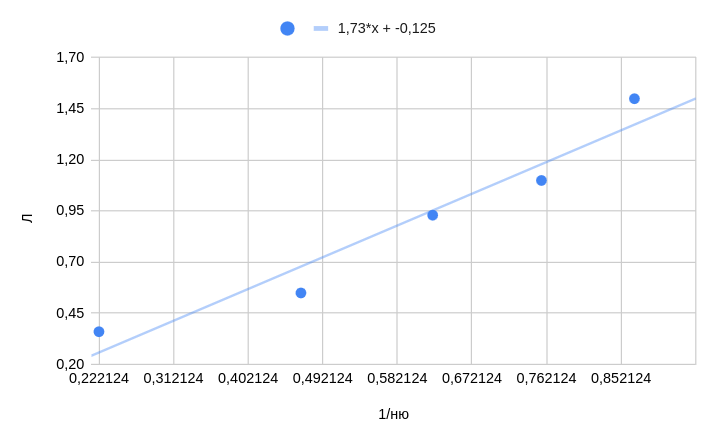
\includegraphics[width=0.9\textwidth]{Images/plot_4.png}
    	\label{shema1}
\end{figure}

\subsection*{Качественные наблюдения}
При закрытии проволкой максимума с номером, отличным от 0, наблюдаем, что период картины не меняется, а менется лишь четкость картины. Это связано с тем, что на период влиет лишь расстояние между ближайшими максимума, которые формируют эту картину, а при закрытии одного любого из них, расстояние между ближайшими не меняется.


\section*{Заключение}
\begin{itemize}
    \item Определили скорость ультразвука по дифракционной картине. Полученные результаты совпали с табличными в пределах погрешности.
    \item Определили скорость ультразвука методом тёмного поля. Полученные результаты совпали с табличными в пределах погрешности.
    \item Произвели качественные наблюдения и объяснили полученный результат.
\end{itemize}


\begin{figure}[H]
    	\centering
    	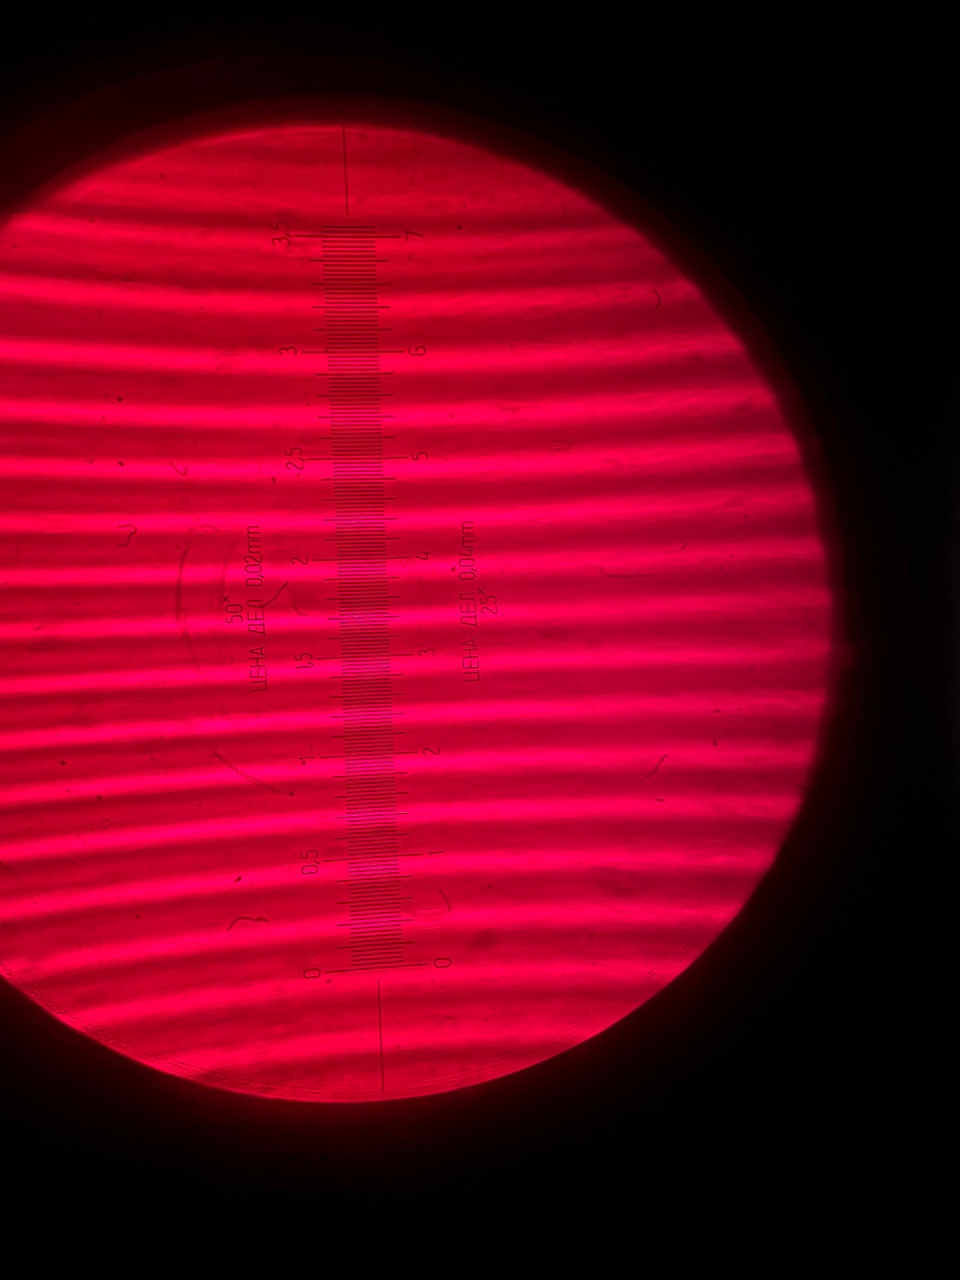
\includegraphics[width=0.6\textwidth]{Images/figure.jpg}
\end{figure}


\end{document}
